\section{Linial's Algorithm}

We now give the description of an algorithm that can be used to merge under
partial information. The merging under partial information problem is the
following,

\begin{problem}
Given a poset \(P\) that can be covered by two chains \(A\) and \(B\), find a
linear extension of \(P\).
\end{problem}

\begin{figure}
\centering
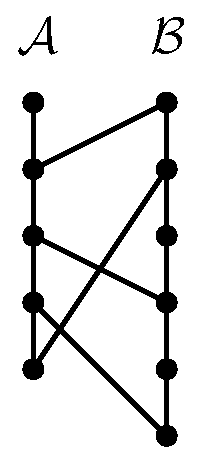
\includegraphics[height=0.2\textheight]{fig/supi/mupi}
\caption{A poset \(P\) covered by two chains \(A\) and \(B\),
input of the MUPI problem.}
\label{fig:supi:mupi}
\end{figure}

\citet*{linial:1984} first proves that the \onethirdtwothird conjecture holds
for width-\(2\) posets, \ie posets that can be covered by two chains. Since one
can always find a good query in \(P\) that when answered will invalidate at
least one third of the possible linear extensions, it is possible to design a
\BigO{\log e(P)} algorithm that solves the MUPI problem.

\begin{theorem}
Given a poset \(P\) covered by two chains \(A\) and \(B\), we can always find
a query \(x \ask{\le} y\) with \(x \in A, y \in B\) such that the probability
that \(x \le y\) lies in the interval \([\sfrac{1}{3}, \sfrac{2}{3}]\).
\end{theorem}

\citet*{linial:1984} proposes the following algorithm. We compute the number of
linear extensions of the width-\(2\) poset \(P\) using the determinant
counting formula. The proof for this determinant counting formula can be found in
\citet*{mohanty:1979}, we give hereunder the statement of this formula when u,

\begin{theorem}
Let \(P = A \cup B\), where \(A = (a_1 \le ))
\end{theorem}


